\normaltrue \difficilefalse \tdifficilefalse
\correctiontrue

%\UPSTIidClasse{11} % 11 sup, 12 spé
%\newcommand{\UPSTIidClasse}{12}

\exer{Barrière Sympact $\star$ \label{C2:06:14}}
\setcounter{question}{0}\UPSTIcompetence[2]{C2-06}
\index{Compétence C2-06}
\index{Barrière Sympact}
\index{Croix de Malte}
\ifcorrection
\else
\marginnote{\textbf{Pas de corrigé pour cet exercice.}}
\fi

\ifprof
\else
Soit le mécanisme suivant. On a $\vect{AC}=H\vect{j_0}$ et $\vect{CB}=R\vect{i_1}$. De plus, 
$H=\SI{120}{mm}$ et $R=\SI{40}{mm}$. 

\begin{center}
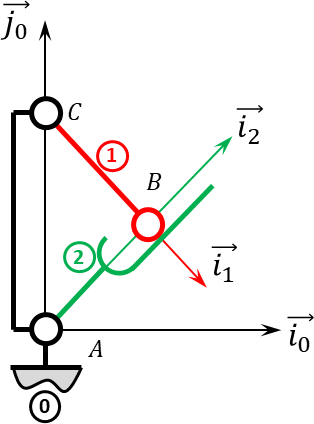
\includegraphics[width=\linewidth]{14_01}
\end{center}
\fi


\question{Tracer le graphe des liaisons.}
\ifprof

\begin{center}
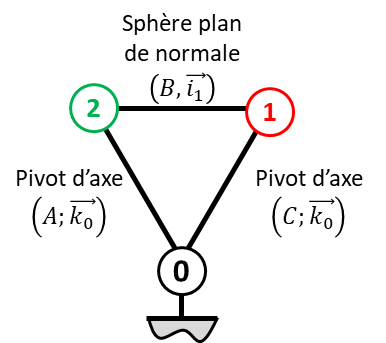
\includegraphics[width=.3\linewidth]{14_01_C}
\end{center}
\else
\fi

\question{Exprimer $ \varphi(t)$ en fonction de $\theta(t)$.}
\ifprof
On a $\vect{AB}+\vect{BC}+\vect{CA}=\vect{0}$ soit 
$\lambda(t)\vi{2}-R\vi{1}-h\vj{0}=\vect{0}$.

En exprimant l'équation vectorielle dans le repère $\rep{0}$, on a 
$\lambda(t)\left( \cos\varphi(t)\vi{0}+\sin\varphi(t)\vj{0}\right)-R\left( \cos\theta(t)\vi{0}+\sin\theta(t)\vj{0}\right)-h\vj{0}=\vect{0}$.

On a alors 
$
\left\{
\begin{array}{l}
\lambda(t)\cos\varphi(t)-R \cos\theta(t)=0 \\
\lambda(t)\sin\varphi(t)-R\sin\theta(t)-h=0
\end{array}
\right.
$

soit 
$
\left\{
\begin{array}{l}
\lambda(t)\cos\varphi(t)=R \cos\theta(t) \\
\lambda(t)\sin\varphi(t)=R\sin\theta(t)+h
\end{array}
\right.
$.

En faisant le rapport des équations, on a donc : $\tan\varphi(t)=\dfrac{R\sin\theta(t)+h}{R \cos\theta(t)}$ (pour $\theta(t)\neq \dfrac{\pi}{2} \, mod \pi$).

\else
\fi

\question{Exprimer $\dot{\varphi}(t)$ en fonction de $\dot{\theta}(t)$.}
\ifprof
On a : $ \varphi(t)=\arctan \left( \dfrac{R\sin\theta(t)+h}{R \cos\theta(t)}\right)$.

Pour commencer, $\left( R\sin\theta(t)+h\right)'$ $=R\thetap(t)\cos\theta(t) $
et $\left( R \cos\theta(t)\right)'$ $=- R \thetap(t)\sin\theta(t)$.

De plus, 
$\left( \dfrac{R\sin\theta(t)+h}{R \cos\theta(t)}\right)'$

$ = \dfrac{R\thetap(t)\cos\theta(t) R \cos\theta(t) + R \thetap(t)\sin\theta(t) \left( R\sin\theta(t)+h\right) }{ R^2 \cos^2\theta(t)}$

$ = \dfrac{R^2\thetap(t)\cos^2\theta(t)  + R \thetap(t)\sin\theta(t) \left( R\sin\theta(t)+h\right) }{ R^2 \cos^2\theta(t)}$


$ = \dfrac{R\thetap(t)\cos^2\theta(t)  +   R\sin^2\theta(t)\thetap(t)+h\thetap(t)\sin\theta(t)}{ R \cos^2\theta(t)}$

$ = \thetap(t)\dfrac{R+h\sin\theta(t)}{ R \cos^2\theta(t)}$.


Au final, 

$ \varphip(t) =  \dfrac{\thetap(t)\dfrac{R+h\sin\theta(t)}{ R \cos^2\theta(t)}}{1+\left( \dfrac{R\sin\theta(t)+h}{R \cos\theta(t)}\right)^2}$
$   \dfrac{\thetap(t)\dfrac{R+h\sin\theta(t)}{ R \cos^2\theta(t)}}{1+ \dfrac{\left(R\sin\theta(t)+h\right)^2}{R^2 \cos^2\theta(t)}}$.

$ \varphip(t) =  R^2 \cos^2\theta(t) \dfrac{\thetap(t)\dfrac{R+h\sin\theta(t)}{ R \cos^2\theta(t)}}{R^2 \cos^2\theta(t)+ \dfrac{\left(R\sin\theta(t)+h\right)^2}{R^2 \cos^2\theta(t)}}$
$ =  \dfrac{R \thetap(t)\left(R+h\sin\theta(t)\right)}{R^2 \cos^2\theta(t)+ \left(R\sin\theta(t)+h\right)^2}$.

$ \varphip(t) =  \dfrac{R \thetap(t)\left(R+h\sin\theta(t)\right)}{R^2 \cos^2\theta(t)+ R^2\sin^2\theta(t)+h^2+2 Rh\sin\theta(t)}$
$ =  \dfrac{R \thetap(t)\left(R+h\sin\theta(t)\right)}{R^2+h^2+2 Rh\sin\theta(t)}$.

\else
\fi

\question{En utilisant Python, tracer $\dot{\varphi}(t)$ en fonction de $\dot{\theta}(t)$. On considérera que la fréquence de rotation de la pièce \textbf{1} est de 10 tours par minute.}
\ifprof

\begin{center}
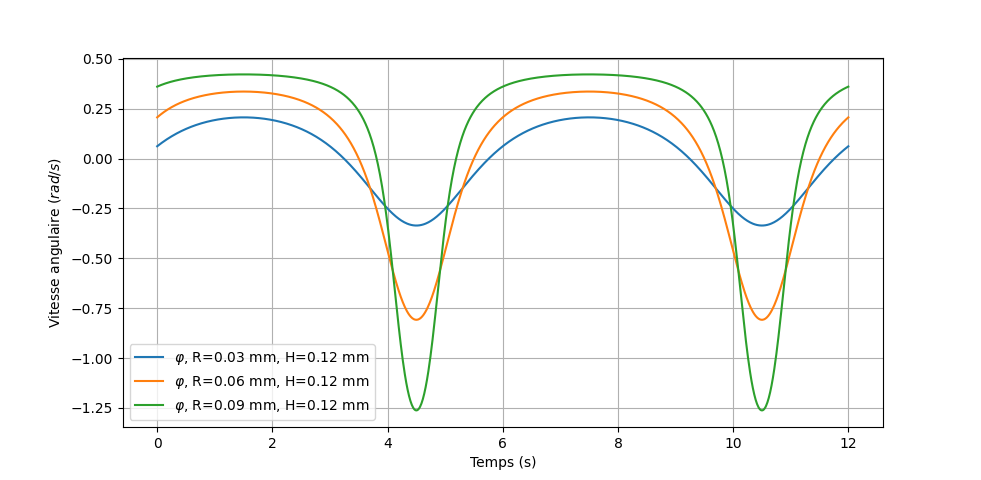
\includegraphics[width=.7\linewidth]{14_02_c}
\end{center}

\noindent\hrule
\begin{lstlisting}
#!/usr/bin/env python
# -*- coding: utf-8 -*-

"""14_Sympact.py"""

__author__ = "Xavier Pessoles"
__email__ = "xpessoles.ptsi@free.fr"

import numpy as np
import matplotlib.pyplot as plt
import math as m
from scipy.optimize import newton
from scipy.optimize import fsolve

R = 0.03 # m
H = 0.12     # m
w = 10 # tours /min
w = 10*2*m.pi/60  # rad/s

def calc_phi(theta):
    num = R*np.sin(theta)+H
    den = R*np.cos(theta)
    return np.arctan2(num,den)

def calc_phip(theta):
    num = R*w*(R+H*np.sin(theta))
    den = R*R+H*H+2*R*H*np.sin(theta)
    return np.arctan2(num,den)

def plot_phi():
    les_t = np.linspace(0,12,1000)
    les_theta = w*les_t
    les_phi = calc_phi(les_theta)
    plt.grid()
    plt.xlabel("Temps (s)")
    plt.ylabel("Position angulaire ($rad$)")
    #plt.plot(les_t,les_theta,label=str("$\\theta$, R=")+str(R)+" mm,"+str("H=")+str(H)+" mm")
    plt.plot(les_t,les_phi,label=str("$\\varphi$, R=")+str(R)+" mm, "+str("H=")+str(H)+" mm")
    plt.legend()
    plt.show()


def plot_phip():
    les_t = np.linspace(0,12,1000)
    les_theta = w*les_t
    les_phip = calc_phip(les_theta)
    
    plt.grid()
    plt.xlabel("Temps (s)")
    plt.ylabel("Vitesse angulaire ($rad/s$)")
    #plt.plot(les_t,les_theta,label=str("$\\theta$, R=")+str(R)+" mm,"+str("H=")+str(H)+" mm")
    plt.plot(les_t,les_phip,label=str("$\\varphi$, R=")+str(R)+" mm, "+str("H=")+str(H)+" mm")
    plt.legend()
    plt.show()

for R in [0.03,0.06,0.09]:
    plot_phip()
\end{lstlisting}
\noindent\hrule

\else
\fi


\ifprof
\else
\footnotesize
\ifcolle
\else
\begin{center}
\begin{tabular}{|p{.9\linewidth}|}
\hline
Indications :
\begin{enumerate}
\item .
\item $\tan\varphi(t)=\dfrac{R\sin\theta(t)+h}{R \cos\theta(t)}$.
\item $ \varphip(t) =  \dfrac{R \thetap(t)\left(R+h\sin\theta(t)\right)}{R^2+h^2+2 Rh\sin\theta(t)}$.
\item .
\end{enumerate} \\ \hline
\end{tabular}
\end{center}
\fi
\normalsize
\begin{flushright}
\footnotesize{Corrigé  voir \ref{C2:06:14}.}
\end{flushright}%
\fi